 \documentclass[a4paper,12pt]{article}
%%%%%%%%%%%%%%%%%%%%%%%%%%%%%%%%%%%%%%%%%%%%%%%%%%%%%%%%%%%%%%%%%%%%%%%%%%%%%%%%%%%%%%%%%%%%%%%%%%%%%%%%%%%%%%%%%%%%%%%%%%%%%%%%%%%%%%%%%%%%%%%%%%%%%%%%%%%%%%%%%%%%%%%%%%%%%%%%%%%%%%%%%%%%%%%%%%%%%%%%%%%%%%%%%%%%%%%%%%%%%%%%%%%%%%%%%%%%%%%%%%%%%%%%%%%%
\usepackage{eurosym}
\usepackage{vmargin}
\usepackage{amsmath}
\usepackage{framed}
\usepackage{multicol}
\usepackage{graphics}
\usepackage{enumerate}
\usepackage{epsfig}
\usepackage{subfigure}
\usepackage{fancyhdr}

\setcounter{MaxMatrixCols}{10}
%TCIDATA{OutputFilter=LATEX.DLL}
%TCIDATA{Version=5.00.0.2570}
%TCIDATA{<META NAME="SaveForMode" CONTENT="1">}
%TCIDATA{LastRevised=Wednesday, February 23, 2011 13:24:34}
%TCIDATA{<META NAME="GraphicsSave" CONTENT="32">}
%TCIDATA{Language=American English}

\pagestyle{fancy}
\setmarginsrb{20mm}{0mm}{20mm}{25mm}{12mm}{11mm}{0mm}{11mm}
\lhead{MA4413 2013} \rhead{Mr. Kevin O'Brien}
\chead{Addition to Formula Sheet }
%\input{tcilatex}

\begin{document}

\large 
\noindent \textbf{Entropies: Example (a)}
\begin{itemize}
\item The input source to a noisy communication channel is a random variable X over the
four symbols $\{a, b, c, d\}$. \item  The output from this channel is a random variable Y over these same
four symbols.
\end{itemize}

\medskip 
%----------------------------------------------------------------Part 2 %

%% - \noindent \textbf{Entropies: Example (b)}
\noindent The joint distribution of these two random variables is as follows:\\ \bigskip
\begin{center}
\begin{tabular}{|c|c|c|c|c|}
\hline
&x=a& x=b & x=c & x=d \\ \hline
y=a &1/8 &1/16 &1/16 &1/4 \\ \hline
y=b &1/16 & 1/8& 1/16& 0 \\ \hline
y=c & 1/32&1/32 & 1/16 & 0\\ \hline
y=d & 1/32& 1/32& 1/16 & 0\\ \hline 
\end{tabular}
\end{center}

%----------------------------------------------------------------Part 2 %

\noindent \textbf{Exercises}
\begin{enumerate}[(a)]
 \item Write down the marginal distribution for $X$ and compute the marginal entropy $H(X)$.
\item Write down the marginal distribution for $Y$ and compute the marginal entropy $H(Y )$.
\item What is the joint entropy $H(X, Y ) $ of the two random variables?
\item What is the conditional entropy $H(Y|X)$?
\item What is the conditional entropy $H(X|Y)$?
\item What is the mutual information $I(X;Y)$ between the two random variables?
\end{enumerate}


\newpage 

\noindent \textbf{Parts (a) and (b)}\\
The marginal distribution of these two random variables is as follows:\\ \bigskip
{
\Large 
\begin{center}
\begin{tabular}{|c|c|c|c|c||c|}
\hline
&x=a& x=b & x=c & x=d &\textbf{P(Y)}\\ \hline
y=a &1/8 &1/16 &1/16 &1/4 & \textbf{0.50}\\ \hline
y=b &1/16 & 1/8& 1/16& 0 & \textbf{0.25}\\ \hline
y=c & 1/32&1/32 & 1/16 & 0& \textbf{0.125}\\ \hline
y=d & 1/32& 1/32& 1/16 & 0& \textbf{0.125}\\ \hline \hline
\textbf{P(X)} & \textbf{0.25}& \textbf{0.25}& \textbf{0.25} & \textbf{0.25}&\\ \hline
\end{tabular}
\end{center}
}
\medskip
\begin{itemize}
\item $H(X)$, the entropy of $X$, is computed as\\
 \[H(X) = -\sum P(x_i) \mbox{log}_2P(x_i)\] \item $H(X) =  (-0.25 \times -2) + (-0.25 \times -2) +(-0.25 \times -2) +(-0.25 \times -2)$\item $ H(X) = 2 \mbox{b}$ \bigskip

\item H(X) , the entropy of Y, is computed as\\
 \[H(Y) = -\sum P(y_j) \mbox{log}_2P(y_j)\] \item $H(Y) =  (-0.5 \times -1) +(-0.25 \times -2)  + (-0.125 \times -3)  +(-0.125 \times -3)$\item $ H(Y) = 1.75 \mbox{b}$



\end{itemize}

\newpage 

\noindent \textbf{Part (c)}
\begin{itemize}

\item To compute the joint entropy $H(X,Y)$,  we will use \[H(X,Y) = -\sum P(x_i,y_y) \mbox{log}_2P(x_i,y_j)\]

\item This means we should compute the entropy component for each cell of the table, and sum up all the resultant terms.
\bigskip
\item To save time, we will aggregate similar results, 
\begin{itemize} 
\item[$\ast$] there are 4 cells where the probability is $1/32$,
\item[$\ast$] 6 cells with probability $1/16$, 
\item[$\ast$] 2 cells with probability $1/8$
\item[$\ast$] and 1 cell with probability $1/4$. 
\end{itemize}
\item Solving
\[ H(X,Y) = [4 \times -{1\over 32} \mbox{log}_2 {1\over 32} ] + [6 \times -{1\over 16} \mbox{log}_2 {1\over 16} ] + \ldots + [1 \times -{1\over 4} \mbox{log}_2 {1\over 4} ] \]

\item Simplifying\[ H(X,Y) = [4 \times -{1\over 32} \mbox{log}_2 {1\over 32} ] + [6 \times -{1\over 16} \mbox{log}_2 {1\over 16} ] + \ldots + [1 \times -{1\over 4} \mbox{log}_2 {1\over 4} ] \]
\item Simplifying \[H(X,Y) = [-{4\over 32} \times -5 ] + [-{6\over 16} \times -4 ] + [-{2\over 8} \times -3 ] + [ -{1\over 4} \times -2]\]
\item $H(X,Y) = 27/8$ b.
\end{itemize}

%---------------------------------------------------------------------------------------------------------------------------------------%
\newpage
\noindent \textbf{Parts (d) and (e)}
\begin{framed}
\noindent Two useful relationships among the types of entropies are
\begin{itemize}
\item $H(X,Y)=H(X|Y)+H(Y) $
\item $H(X,Y)=H(Y|X)+H(X) $
\end{itemize}
\bigskip
Re-arranging these formulae
\begin{itemize}
\item $H(X,Y)-H(Y) = H(X|Y) $
\item $H(X,Y)-H(X) = H(Y|X) $
\end{itemize}
\end{framed}

%---------------------------------------------------------------------------------------------------------------------------------------%



\noindent Re-arranging these formulae
\begin{itemize}
\item $H(X|Y) = H(X,Y)-H(Y) = 27/8 - 14/8 = 13/8$ b. \bigskip
\item $H(Y|X) = H(X,Y)-H(X) = 27/8 - 16/8 = 11/8$ b.
\end{itemize}
\bigskip
\begin{itemize}
\item Remark $1.75 =14/8$ and $2 = 16/8$.\\\bigskip
%\item Also: we will derive $H(Y|X$ and $H(X|Y)$ from first principles in a tutorial.
\end{itemize}

%---------------------------------------------------------------------------------------------------------------------------------------%

\newpage 
\noindent \textbf{Part (f)}\\
There are three alternative ways to obtain the answer:
\begin{eqnarray*}
I(X; Y ) &=& H(X) + H(Y ) - H(X,Y )\\ 
&=& 2 + \frac{7}{4} - \frac{27}{8} \\
&=& \frac{16+14-27}{8} \\
&=& 3/8 \mbox{ b}.\\
\end{eqnarray*}

\begin{center}
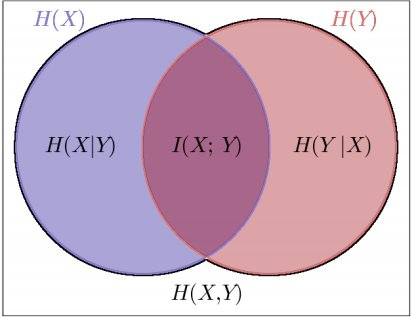
\includegraphics[scale=0.8]{images/11BMutualInfo.jpg}
\end{center}

\begin{itemize}
\item $I(X; Y ) = H(Y ) - H(Y |X)$ = $7/4 - 11/8 = 3/8$ b.
\item $I(X; Y ) = H(X) - H(X|Y)$ = $2 - 13/8 = 3/8$ b.

\end{itemize}

\end{document}